\documentclass[conference]{IEEEtran}
\IEEEoverridecommandlockouts

\usepackage{cite}
\usepackage{amsmath}
\usepackage{graphicx}
\usepackage{booktabs}
\usepackage{array}
\usepackage{url}
\usepackage{textcomp}
\usepackage{xcolor}
\usepackage{tikz}
\usetikzlibrary{arrows.meta,positioning,shapes.geometric,fit,calc}

\def\BibTeX{{\rm B\kern-.05em{\sc i\kern-.025em b}\kern-.08em
    T\kern-.1667em\lower.7ex\hbox{E}\kern-.125em X}}

\newcommand{\code}[1]{\texttt{\small #1}}

\begin{document}

\title{Resilient TaskFlow: A Crash-Safe Job Processing System Using a Transactional Outbox, Lease Fencing, and Redis Streams}

\author{\IEEEauthorblockN{Pankaj Baid}
\IEEEauthorblockA{baidpankaj567@gmail.com}}

\maketitle

\begin{abstract}
Asynchronous job systems commonly lose jobs when a process crashes between saving a job and queueing it, or run a job twice after a worker dies. Resilient TaskFlow is a TypeScript job queue that keeps PostgreSQL as the only source of truth and uses Redis Streams only to notify workers. It combines a transactional outbox, time-limited leases with fencing, acknowledgement after commit, and a priority window ordered in PostgreSQL. Delivery is at-least-once, so handlers must make external effects idempotent. We describe the design, map each failure scenario to an automated test, and report measurements from a single laptop. One API process admitted 500 jobs/s with a 346~ms p99 and no errors. Draining a 20{,}000-job backlog reached about 200 to 250 jobs/s regardless of worker count because PostgreSQL was the bottleneck. After a \code{SIGKILL} of one of two workers, no job was lost and 8 of 10{,}000 jobs were re-run after the 30~s lease; after \code{SIGTERM}, none consumed an extra attempt. Benchmarking also exposed three defects that we fixed. These are single-machine results, not production capacity.
\end{abstract}

\begin{IEEEkeywords}
job queue, transactional outbox, lease fencing, at-least-once delivery, PostgreSQL, Redis Streams, fault tolerance
\end{IEEEkeywords}

%--------------------------------------------------------------------
\section{Introduction}
Background work such as sending email or processing uploads is usually handed to a queue. Two failures recur in practice. First, a service writes a job to its database and then publishes it to a broker; a crash between the two leaves a job that is saved but never runs. Second, a worker takes a job, crashes, and the job is either lost (the broker already removed it) or run again with no record that a first attempt happened.

Resilient TaskFlow addresses both with a deliberately small set of mechanisms and tests each against real PostgreSQL and Redis processes. The contributions are:
\begin{itemize}
  \item A design in which PostgreSQL alone decides job state, and a \emph{transactional outbox} makes ``job saved'' and ``job will be delivered'' a single atomic fact (Section~\ref{sec:design}).
  \item \emph{Fenced leases} and acknowledgement only after a terminal commit, so a worker that lost its lease cannot overwrite a newer result, and a crash after commit does not re-run the handler.
  \item A \emph{priority window}: the backlog stays in PostgreSQL ordered by priority, and only a bounded number of entries are placed in each FIFO Redis stream.
  \item A shutdown path that hands leases back and refunds the attempt, so deployments do not consume retry budget.
  \item A failure model in which every scenario is tied to an automated test (Section~\ref{sec:failure}), and a measured evaluation with its limits stated (Section~\ref{sec:eval}), including three defects the benchmarks found.
\end{itemize}
The system guarantees at-least-once execution. It does not provide exactly-once effects on external systems, and we do not claim it.

%--------------------------------------------------------------------
\section{Background and Related Work}
\subsection{Delivery guarantees}
At-most-once delivery can lose work; exactly-once effects across a queue and an external system require the receiver to deduplicate. Queue systems therefore generally offer at-least-once delivery and ask handlers to be idempotent. Celery's documentation states this directly for late acknowledgement: a task that already started will be retried after an abrupt worker failure, so it must be idempotent~\cite{celeryoptimizing}.

\subsection{Building blocks}
\textbf{Transactional outbox.} Instead of writing to a database and a broker separately, the service writes the message into an outbox table in the same transaction as the state change, and a separate relay publishes it~\cite{richardson2018patterns}. This follows the general argument that coordination across separate stores should be built from idempotent messages rather than distributed transactions~\cite{helland2007beyond}.

\textbf{Leases.} A lease grants exclusive rights for a bounded time and expires on its own if the holder fails~\cite{gray1989leases}. A lease alone does not stop a slow holder from acting after it expired; a monotonically checked token (\emph{fencing}) in the write does~\cite{kleppmann2017ddia}.

\textbf{Redis Streams.} Streams with consumer groups give each entry to one consumer and keep it in a pending list until acknowledged. \code{XAUTOCLAIM} transfers entries idle longer than a threshold to another consumer, and claiming resets the idle time so one consumer wins~\cite{redisstreams,redisxautoclaim}.

\textbf{\code{SKIP LOCKED}.} PostgreSQL's \code{SELECT \ldots FOR UPDATE SKIP LOCKED} skips rows that cannot be locked immediately. The documentation notes the view is inconsistent, so it is unsuitable for general work, but it avoids lock contention among consumers of a queue-like table~\cite{pgselect}.

\subsection{Existing systems}
Table~\ref{tab:related} summarises documented behaviour of widely used systems on the points TaskFlow is built around. It is limited to statements in the cited documentation and is not a performance comparison; we ran no benchmark of the other systems.

\begin{table*}[t]
\caption{Documented behaviour of related systems (from the cited documentation only).}
\label{tab:related}
\centering
\small
\begin{tabular}{p{1.9cm}p{4.3cm}p{4.6cm}p{4.6cm}}
\toprule
System & Where job state lives & Recovery after worker crash & Priority \\
\midrule
Celery with Redis~\cite{celeryredis,celeryoptimizing} & Broker holds the message until acknowledged; results in an optional backend & Unacknowledged message is redelivered after the visibility timeout (default 1 hour for Redis) & Not covered here \\
Sidekiq~\cite{sidekiqreliability} & Redis lists; basic fetch removes the job with \code{BRPOP} & Basic fetch can lose a job if the process crashes; Pro \code{super\_fetch} keeps jobs in Redis and recovers orphans after heartbeat expiry & Queue order: strict (may starve) or weighted random \\
BullMQ~\cite{bullmqstalled,bullmqprio} & Redis & Jobs that stop renewing are moved back to waiting (a \emph{stalled} job); failed after \code{maxStalledCount} (default 1) & Prioritized set; documented insertion cost $O(\log n)$ \\
Temporal~\cite{temporalhistory,temporalactivity} & Event History persisted by the Temporal service in a database & Activities retry by default with exponential backoff; a completed activity is not re-executed on replay & Not covered here \\
TaskFlow (this work) & PostgreSQL; Redis only notifies & Fenced lease expiry plus pending-entry reclaim; outbox republish & Priority ordered in PostgreSQL before a bounded Redis window \\
\bottomrule
\end{tabular}
\end{table*}

%--------------------------------------------------------------------
\section{System Design}
\label{sec:design}

\subsection{Architecture}
Fig.~\ref{fig:arch} shows the components. The API authenticates callers (database-backed API keys or signed JWTs), rate-limits per user and validates input. Workers run four loops in one process: a \emph{dispatcher} that moves outbox rows to Redis, a \emph{worker pool} that executes jobs, a \emph{scheduler} that promotes delayed jobs, and a \emph{retention} task that deletes old data. Prometheus scrapes the API and every worker.

\begin{figure*}[t]
\centering
\resizebox{0.98\textwidth}{!}{%
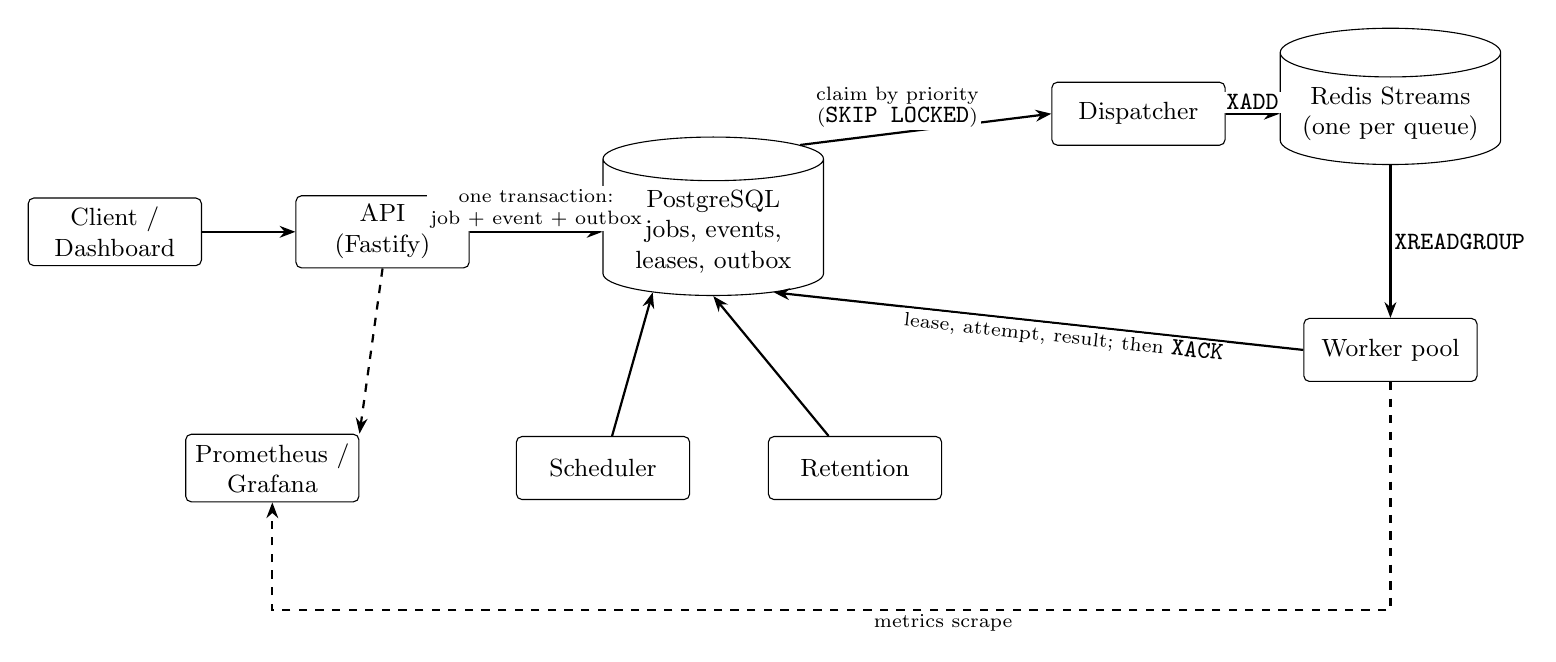
\begin{tikzpicture}[
  box/.style={draw, rounded corners=2pt, minimum height=8mm, minimum width=22mm, align=center, font=\small},
  store/.style={draw, cylinder, shape border rotate=90, aspect=0.25, minimum height=14mm, minimum width=28mm, align=center, font=\small},
  arr/.style={-{Stealth[length=2mm]}, thick},
  lbl/.style={font=\scriptsize, align=center, fill=white, inner sep=1pt}
]
\node[box] (client) at (0,0) {Client /\\Dashboard};
\node[box] (api) at (3.4,0) {API\\(Fastify)};
\node[store] (pg) at (7.6,0) {PostgreSQL\\jobs, events,\\leases, outbox};
\node[box] (disp) at (13.0,1.5) {Dispatcher};
\node[store] (redis) at (16.2,1.5) {Redis Streams\\(one per queue)};
\node[box] (pool) at (16.2,-1.5) {Worker pool};
\node[box] (sched) at (6.2,-3.0) {Scheduler};
\node[box] (ret) at (9.4,-3.0) {Retention};
\node[box] (prom) at (2.0,-3.0) {Prometheus /\\Grafana};

\draw[arr] (client) -- (api);
\draw[arr] (api) -- node[lbl, above] {one transaction:\\job + event + outbox} (pg);
\draw[arr] (pg.north east) -- node[lbl, above, pos=0.45, xshift=-2mm] {claim by priority\\(\code{SKIP LOCKED})} (disp.west);
\draw[arr] (disp) -- node[lbl, above] {\code{XADD}} (redis);
\draw[arr] (redis) -- node[lbl, right] {\code{XREADGROUP}} (pool);
\draw[arr] (pool.west) -- node[lbl, below, sloped, pos=0.45] {lease, attempt, result; then \code{XACK}} (pg.south east);
\draw[arr] (sched) -- (pg.south west);
\draw[arr] (ret) -- (pg.south);
\draw[arr, dashed] (api.south) -- (prom.north east);
\draw[arr, dashed] (pool.south) -- ++(0,-2.9) -| node[lbl, below, pos=0.2] {metrics scrape} (prom.south);
\end{tikzpicture}}
\caption{Architecture. Solid arrows are the data path; dashed arrows are metrics scrapes. Redis holds no state that cannot be rebuilt from PostgreSQL.}
\label{fig:arch}
\end{figure*}

\subsection{Data model}
The central tables are \code{jobs} (status, attempts, version, lease id and expiry, priority), \code{job\_attempts}, \code{job\_events} (append-only history), \code{job\_deliveries} (the outbox), \code{workers}, \code{dead\_letter\_jobs}, \code{idempotency\_keys}, \code{api\_keys} and an operational audit log. Ten SQL migrations create them and are applied under an advisory lock with recorded checksums.

\subsection{State machine}
A job moves through the states in Fig.~\ref{fig:states}. The transition table is a single constant that is checked before every status \code{UPDATE} (12 call sites), and a contract test pins the table to the transitions the repositories actually perform. \code{SUCCEEDED}, \code{CANCELLED} and \code{DEAD\_LETTERED} are terminal. A \code{FAILED} state remains defined only for legacy rows.

\begin{figure}[t]
\centering
\resizebox{\columnwidth}{!}{%
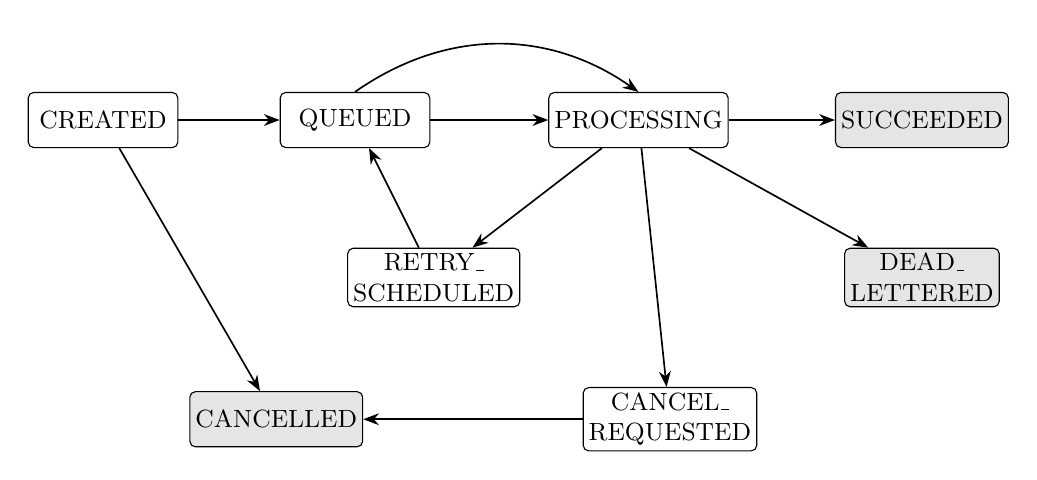
\begin{tikzpicture}[
  st/.style={draw, rounded corners=2pt, font=\small, minimum height=7mm, minimum width=19mm, inner sep=2pt, align=center},
  term/.style={st, fill=gray!20},
  arr/.style={-{Stealth[length=2mm]}, semithick}
]
\node[st] (created) at (0,0) {CREATED};
\node[st] (queued) at (3.2,0) {QUEUED};
\node[st] (proc) at (6.8,0) {PROCESSING};
\node[term] (succ) at (10.4,0) {SUCCEEDED};
\node[st] (retry) at (4.2,-2.0) {RETRY\_\\SCHEDULED};
\node[term] (dlq) at (10.4,-2.0) {DEAD\_\\LETTERED};
\node[st] (creq) at (7.2,-3.8) {CANCEL\_\\REQUESTED};
\node[term] (canc) at (2.2,-3.8) {CANCELLED};

\draw[arr] (created) -- (queued);
\draw[arr] (queued) -- (proc);
\draw[arr] (proc) -- (succ);
\draw[arr] (proc) -- (retry);
\draw[arr] (retry) -- (queued);
\draw[arr] (proc) -- (dlq);
\draw[arr] (proc) -- (creq);
\draw[arr] (creq) -- (canc);
\draw[arr] (created) -- (canc);
\draw[arr] (queued.north) to[bend left=35] (proc.north);
\end{tikzpicture}}
\caption{Job states (main transitions). \code{QUEUED}, \code{CREATED} and \code{RETRY\_SCHEDULED} can also be cancelled directly, and \code{CANCEL\_REQUESTED} may still end in \code{SUCCEEDED} if the handler finishes first. The ``lease handed back'' arrow is \code{PROCESSING}$\rightarrow$\code{QUEUED}.}
\label{fig:states}
\end{figure}

\subsection{Submission and the outbox}
In one PostgreSQL transaction the API inserts the job, its \code{created}/\code{queued} events and a \code{PENDING} row in \code{job\_deliveries}. The API never writes the job to Redis, so a crash cannot leave a saved job without a delivery intent. An optional \code{Idempotency-Key} is checked in the same transaction under a transaction-scoped advisory lock~\cite{pglocking}: the same key and body replays the first response, and a different body returns \code{409}.

\subsection{Dispatch and the priority window}
\label{sec:window}
The dispatcher claims due outbox rows with \code{FOR UPDATE SKIP LOCKED} and a persisted claim lease that expires if the dispatcher dies, publishes them with \code{XADD}, and records the Redis message id. A Redis stream is FIFO, so ordering must be applied \emph{before} publishing. Each row stores a \code{priority\_rank} computed on insert by a SQL function (so there is one definition of the order), and a partial index on \code{(queue, rank DESC, available\_at, created\_at)} serves the claim. Per queue and per cycle the dispatcher computes $\text{budget}=W-\text{inflight}$, where $W$ is the window (default 200) and \emph{inflight} is pending plus undelivered entries of the consumer group, and claims at most that many rows, highest priority first. A late \code{CRITICAL} job therefore waits behind at most the window rather than the whole backlog. The window is soft: concurrent dispatchers can overshoot by one batch each, ordering is strict with no aging, and nothing is preempted.

\subsection{Leases, fencing and commit before acknowledgement}
A worker reads an entry and then acquires a lease on the job in PostgreSQL, writing a lease id and an expiry and creating an attempt. The lease is renewed at one third of its duration (30~s by default) and renewals write no events. Every result commit checks the lease id and the job version in the same transaction, so a worker whose lease expired cannot overwrite a newer outcome. The worker sends \code{XACK} only after the terminal state is committed. If it crashes in between, the entry is redelivered and the next worker finds the job already terminal and only acknowledges it, without re-running the handler.

\subsection{Recovery}
Entries left pending by a dead worker are claimed by another consumer once idle longer than the lease duration (\code{XAUTOCLAIM}). Independently, the dispatcher republishes deliveries that are marked published but whose job is not terminal after 120~s, which covers loss of Redis data. Outbox claims abandoned by a dead dispatcher become claimable again after a timeout.

\subsection{Retries, dead letters and cancellation}
Failures are classified as retriable or permanent. A retriable failure schedules a successor outbox row available after an exponentially growing, capped delay, and the job returns to \code{QUEUED}; a permanent failure or exhausted attempts moves it to \code{DEAD\_LETTERED} with a dead-letter record, from which an owner may create one replacement job. Cancellation of a running job sets \code{CANCEL\_REQUESTED} and signals a cooperative token. If the handler finishes at the same moment, the first durable observation wins, and a failure reported while cancellation is requested makes the worker complete the cancellation instead of scheduling a retry.

\subsection{Scheduling, shutdown and retention}
Delayed jobs are created in \code{CREATED} and promoted by the scheduler using \code{SKIP LOCKED} so concurrent schedulers handle disjoint rows. On \code{SIGTERM} a worker stops taking work, waits for running handlers up to a timeout and then hands each unfinished lease back in a fenced transaction: the job returns to \code{QUEUED}, the in-flight attempt is refunded, the outbox row is re-armed and a \code{lease\_released} event is written. Without the refund a rolling deployment would spend one attempt per running job. Retention runs in every worker but is serialised by a Redis lock; it deletes terminal jobs and their history in bounded \code{SKIP LOCKED} batches, never touches data of a live job, and trims streams without passing the oldest pending entry.

%--------------------------------------------------------------------
\section{Implementation}
The system is a pnpm and Turborepo TypeScript monorepo. The API uses Fastify; persistence uses Drizzle ORM over postgres.js with hand-written SQL migrations; Redis access uses ioredis, with a second connection reserved for blocking reads (Section~\ref{sec:eval}). Metrics use prom-client, with optional OpenTelemetry tracing, and the dashboard is a React single-page application served by nginx. Measured with \code{wc -l}, the repository has 18{,}399 lines in 109 TypeScript/TSX source files (including 2{,}743 in the dashboard) and 10{,}271 lines in 37 test files, plus 736 lines of SQL in 10 migrations. There are 266 unit tests (plus 15 database contract tests that need PostgreSQL) and 46 Docker integration tests.

%--------------------------------------------------------------------
\section{Failure Model and Correctness}
\label{sec:failure}
Table~\ref{tab:failure} lists the failure scenarios, the intended behaviour and the integration test that exercises each. The tests start real worker processes against Dockerised PostgreSQL and Redis and inspect database rows and \code{XPENDING} directly; the names are prefixes of the test titles in \code{tests/integration/worker-runtime.test.ts}.

\begin{table*}[t]
\caption{Failure scenarios and the integration tests that cover them.}
\label{tab:failure}
\centering
\small
\begin{tabular}{p{4.0cm}p{5.4cm}p{6.6cm}}
\toprule
Scenario & Behaviour & Test (title prefix) \\
\midrule
No worker is running & Job stays in the outbox until a worker starts & \emph{retains an API-created job in the database outbox until a worker starts} \\
Normal path & Terminal state committed before \code{XACK} & \emph{takes an API-created job through the shared envelope to durable SUCCEEDED before XACK} \\
Redis entry lost & Dispatcher republishes the non-terminal job & \emph{redispatches a published nonterminal job after its Redis entry is lost} \\
Worker \code{SIGKILL} mid-job & Entry reclaimed; handler may run twice; one idempotent effect & \emph{recovers a pending execution after SIGKILL with duplicate execution but one idempotent effect} \\
Crash after commit, before \code{XACK} & Replacement acknowledges without re-running the handler & \emph{recognizes a result committed before crash and replacement-ACKs without rerunning the handler} \\
Database failure during lease acquisition & Delivery stays pending and later completes & \emph{leaves a delivery pending during transient lease-database failure and later completes it} \\
\code{SIGTERM} with running job & Job drains to \code{SUCCEEDED} before exit & \emph{drains an in-flight job to SUCCEEDED before a SIGTERM-ed worker exits} \\
\code{SIGTERM}, handler ignores cancellation & Lease handed back, attempt budget not consumed & \emph{releases a non-cooperative job on bounded SIGTERM shutdown without consuming its attempt budget} \\
Retries and exhaustion & Exponential delays, dead-letter only after exhaustion & \emph{derives exponential retries from execution and dead-letters only after exhaustion} \\
Retry due while no worker runs & Retry retained through shutdown and idle interval & \emph{retains a due retry through worker shutdown and a workerless interval} \\
Cancellation & Persisted before \code{XACK}; completed by a replacement if the owner is killed & \emph{persists cooperative cancellation before acknowledging the Redis entry}; \emph{lets a replacement terminalize a cancellation request after the owner is killed} \\
Delayed job & Promoted through scheduler and outbox & \emph{promotes a future API-created job through the canonical scheduler and outbox} \\
Priority & Strict priority then age; late \code{CRITICAL} overtakes backlog; FIFO control with window off & \emph{releases a queued backlog strictly by priority, then by age}; \emph{lets a late CRITICAL job overtake a backlog}; \emph{is FIFO without the window} \\
Queue paused & Durable delivery held, resumes later & \emph{holds durable delivery while a queue is paused and resumes processing} \\
Retention & Active leases, pending deliveries and scheduled retries are never purged; one runner at a time & \emph{purges expired terminal jobs while strictly protecting active leases, pending deliveries, and scheduled retries}; \emph{lets exactly one of two concurrent retention schedulers run, using the real Redis lock} \\
\bottomrule
\end{tabular}
\end{table*}

\subsection{Informal invariant argument}
Three properties carry the design. (1) \emph{No due job without a delivery intent:} every transition into \code{QUEUED} (submission, scheduler promotion, retry, release) inserts an outbox row in the same transaction, and the dispatcher keeps trying until a row is published; a published row whose job is not terminal is republished after a delay. (2) \emph{Acknowledge only after a terminal commit:} \code{XACK} follows the commit in the worker, so an entry is never discarded for a job whose outcome was not stored; the converse crash (commit, no \code{XACK}) leads to a redelivery that finds a terminal job. (3) \emph{One effective lease owner:} commits are conditional on the lease id and version, so at most one worker's result is accepted for an attempt even if two believe they hold the job. These are arguments over the code and tests, not a formal proof; the tests cover the listed scenarios, not all interleavings.

%--------------------------------------------------------------------
\section{Evaluation}
\label{sec:eval}
\subsection{Setup}
All numbers come from one Apple M3 laptop (8 cores, 8~GB, macOS 15.6.1) running PostgreSQL 16.15 and Redis 7.4.11 in Docker (8 CPUs, 3.8~GB for the VM), Node.js 20.20.2, the built API and workers, and the k6 2.2.0 load generator on the same machine. One API process used a pool of at most 10 connections; workers ran 20 concurrent jobs each. Rate limits were raised so they did not hide the system. Jobs used either a \code{noop} handler (benchmark-only) or a \code{process-data} handler with about 50~ms of simulated work. Benchmarks used a separate database. The raw commands, scripts and caveats are in the repository (\code{docs/benchmarking/RESULTS.md}).

\subsection{API admission}
Fig.~\ref{fig:adm} and Table~\ref{tab:adm} show \code{POST /api/v1/jobs} at a constant arrival rate for 60~s per rate, with no workers running (this measures the API and the transactional insert, not execution). No request failed at any rate. The stop rule was p99 above 1~s or error rate above 1\%; p99 first exceeded 1~s at 750 requests/s, so the last good rate is 500 requests/s (p99 346~ms). Beyond about 700 requests/s a single API process saturates and achieved throughput falls as the target rises. The p50 at 100 requests/s is higher than at 250 because each run's first seconds include JIT warm-up, which weighs more in a smaller run.

\begin{table}[t]
\caption{API admission (60~s per rate, no workers). Errors were 0 in every run.}
\label{tab:adm}
\centering
\small
\begin{tabular}{rrrrrr}
\toprule
Target & Achieved & p50 & p95 & p99 & Dropped \\
req/s & req/s & ms & ms & ms & iter. \\
\midrule
100 & 100.0 & 7.5 & 19.6 & 74.5 & 0 \\
250 & 249.8 & 3.8 & 27.4 & 135.0 & 10 \\
500 & 497.2 & 3.7 & 200.3 & 345.7 & 165 \\
750 & 728.5 & 243.2 & 1157.7 & 1554.1 & 1033 \\
1000 & 683.4 & 1403.1 & 1900.2 & 2417.1 & 18310 \\
1500 & 546.7 & 1398.3 & 3079.9 & 3943.1 & 55590 \\
\bottomrule
\end{tabular}
\end{table}

\begin{figure}[t]
\centering
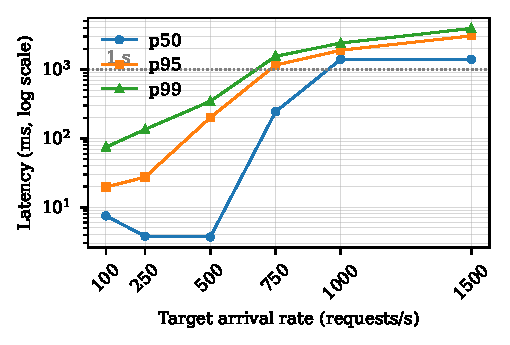
\includegraphics[width=\columnwidth]{figures/admission.pdf}
\caption{Admission latency percentiles versus target arrival rate (log scale).}
\label{fig:adm}
\end{figure}

\subsection{Throughput versus workers}
We enqueued 20{,}000 \code{noop} jobs with no worker running, then started $N$ workers and timed the drain (Fig.~\ref{fig:drain}). Mean throughput over three runs was 221, 241 and 203 jobs/s for 1, 2 and 4 workers. The spread within a configuration (195 to 249) is as large as the difference between configurations, so throughput did not scale with workers on this machine and the ordering of 1 and 2 workers is not significant. With the 50~ms handler and 4 workers (5{,}000 jobs, three runs), throughput was 184, 172 and 214 jobs/s.

PostgreSQL was the limit. During a 2-worker drain the PostgreSQL container used about 260\% CPU while each worker process used about 50\%; with one worker, about 170\% and 77\%. A job costs about 5 transactions, 4 row inserts and 7 updates (database statistics over a 3{,}000-job run), and sampled backends were mostly in \code{commit} or waiting on the client between statements. Setting \code{synchronous\_commit=off} raised a 2-worker run only from about 270 to 297 jobs/s, so commit flushing alone does not explain the plateau. Because the backlog exists before workers start, the created-to-completed latency in these runs (p99 81 to 103~s) measures drain time, not per-job processing time.

\begin{figure}[t]
\centering
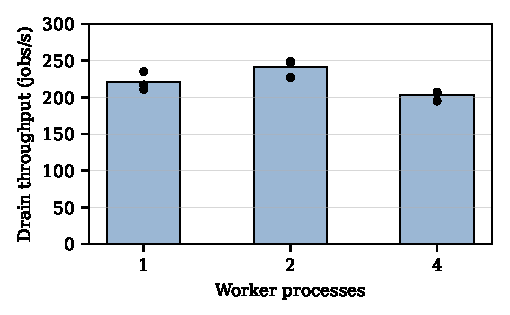
\includegraphics[width=0.95\columnwidth]{figures/drain.pdf}
\caption{Drain throughput of a 20{,}000-job backlog. Bars are means; dots are the three runs.}
\label{fig:drain}
\end{figure}

\subsection{Crash and deployment behaviour}
With 10{,}000 \code{process-data} jobs and two workers, one worker was killed with \code{SIGKILL} after about half the jobs had succeeded. All 10{,}000 jobs finished; none was lost or dead-lettered. Eight jobs were executed twice, each with a \code{lease\_expired} event, and the last re-run finished 30.2~s after the kill, matching the 30~s lease. In the same setup, \code{SIGTERM} of one worker also lost no jobs, no job used more than one attempt, none was dead-lettered, and two jobs were handed back through \code{lease\_released}. Each of these two experiments was run once; the earlier runs on a previous build took longer (about 60~s to finish the remainder) because of a defect described next.

\subsection{Defects found by the benchmarks}
The benchmarks exposed three defects, all fixed before the numbers above were taken.
\begin{enumerate}
  \item \emph{Shared connection.} The consumer's blocking \code{XREADGROUP \ldots BLOCK} shared one Redis connection with the dispatcher's \code{XADD}. Each publish waited for the block to time out, so an idle worker published about 3 jobs/s. Blocking reads now use a dedicated connection. The same 1{,}500-job backlog went from 31 jobs in 10~s to fully drained in under 10~s.
  \item \emph{Fixed sleep at full capacity.} When all concurrency slots were busy the poll loop slept a fixed 250~ms, capping each worker at $20/0.25=80$ jobs/s whatever the handler speed. The loop now wakes when a handler settles; for the 50~ms handler with one worker, throughput rose from about 80 to 224 jobs/s.
  \item \emph{Backlog-sized scan.} Finding which queues had work scanned all pending rows each cycle. It now probes each active queue with \code{EXISTS}. Measured throughput did not change, so this is a cost fix, not a measured speed-up.
\end{enumerate}
Regression tests cover the first two.

%--------------------------------------------------------------------
\section{Limitations and Future Work}
\begin{itemize}
  \item \textbf{External effects.} Delivery is at-least-once. A handler interrupted by a crash runs again, so side effects need their own idempotency keys. Exactly-once sinks are out of scope.
  \item \textbf{Scale evidence.} All measurements are from one machine with shared resources and default PostgreSQL settings. They show where this implementation saturates there, not production capacity, and multi-host scaling is unmeasured. The crash and deployment experiments are single runs.
  \item \textbf{Throughput.} About 5 transactions per job bound throughput on that setup. Batching outbox claims and completion writes, or tuning PostgreSQL, are untested options.
  \item \textbf{Priority.} Ordering is strict without aging, so sustained high-priority load can starve low-priority jobs; there is no preemption and priority is per queue.
  \item \textbf{Operations.} A crashed worker stays \code{ACTIVE} in the database (the dashboard counts only fresh heartbeats). The worker metrics endpoint is unauthenticated and must stay on an internal network. There is one region, no replication or backup procedure, no TLS termination, and the AWS deployment workflow and Terraform are unfinished and unused.
  \item \textbf{Multi-tenancy.} Rate limits are per user, but there is no fairness scheduling between tenants.
\end{itemize}

%--------------------------------------------------------------------
\section{Conclusion}
Keeping PostgreSQL as the single source of truth, writing delivery intent in the same transaction as the job, fencing every result commit with a lease, and acknowledging only after commit gave a system that lost no job in the tested crash scenarios and did not spend retry attempts on graceful shutdown. Ordering a priority backlog in PostgreSQL and exposing only a bounded window to a FIFO stream gave priority without changing the transport. The measurements also showed the cost of this durability on one machine: about 5 transactions per job and a PostgreSQL-bound plateau of roughly 200 to 250 jobs/s, and they found two defects in the worker's use of Redis that functional tests had not exposed.

%--------------------------------------------------------------------
\bibliographystyle{IEEEtran}
\bibliography{references}

\end{document}
